% XeTeX (tectonic): declare Times (TeX Gyre Termes) as TU/ptm before IEEEtran loads,
% so fonts the class preloads at load time are Times rather than a fallback.
\DeclareFontFamily{TU}{ptm}{}
\DeclareFontShape{TU}{ptm}{m}{n}{<->"[texgyretermes-regular.otf]/OT:mapping=tex-text"}{}
\DeclareFontShape{TU}{ptm}{m}{it}{<->"[texgyretermes-italic.otf]/OT:mapping=tex-text"}{}
\DeclareFontShape{TU}{ptm}{b}{n}{<->"[texgyretermes-bold.otf]/OT:mapping=tex-text"}{}
\DeclareFontShape{TU}{ptm}{b}{it}{<->"[texgyretermes-bolditalic.otf]/OT:mapping=tex-text"}{}
\DeclareFontShape{TU}{ptm}{bx}{n}{<->ssub*ptm/b/n}{}
\DeclareFontShape{TU}{ptm}{bx}{it}{<->ssub*ptm/b/it}{}
\DeclareFontShape{TU}{ptm}{m}{sc}{<->ssub*ptm/m/n}{}
\documentclass[conference]{IEEEtran}
\usepackage{iftex}
\ifXeTeX
  \usepackage{fontspec}
  \setmainfont{texgyretermes}[Extension=.otf, UprightFont=*-regular,
    BoldFont=*-bold, ItalicFont=*-italic, BoldItalicFont=*-bolditalic, NFSSFamily=ptm]
\else
  \usepackage[T1]{fontenc}
  \usepackage{mathptmx}
\fi
\usepackage{amsmath,amssymb,amsthm}
\usepackage{graphicx,booktabs,url,xcolor}
\usepackage[hidelinks]{hyperref}
\newtheorem{proposition}{Proposition}
\newcommand{\E}{\mathbb{E}}
\newcommand{\FP}{\mathrm{FP16}}
\newcommand{\Drob}{D_{\mathrm{rob}}}
\newcommand{\TBD}[1]{\textcolor{red}{[#1]}}
\makeatletter
\newcommand{\tableinput}[1]{\@@input #1 }
\makeatother
\title{From Weight Collisions to Behavior:\\Auditing Quantized Concept Erasure in Diffusion Models}
\author{\IEEEauthorblockN{Anonymous Authors}}
\begin{document}
\maketitle

\begin{abstract}
Can post-training quantization undermine concept erasure in diffusion models?
A supplier could ship weights that appear erased in full precision but whose
quantized form is the unedited model. We characterize scale-preserving collisions
for erasers that edit cross-attention key and value maps. Because those maps see only
text embeddings, generated images depend on the edit solely through its key/value
outputs. The full collision set is a union of boxes; within the box that retains the
original arg-max coordinates, a convex program certifies the best reconstruction of
this edit's key/value outputs, not optimal behavioral stealth. On Stable Diffusion 1.5
with UCE erasure of Van Gogh style and nudity, the constructed 8-bit checkpoints,
with or without SmoothQuant, reproduce 34--42\% of the erasure's measured key/value
effect and score like the unedited model in FP16. At 4 bits (INT4 and NF4), the
constructed checkpoints show substantial recovery: with 192 images
per condition from 12 crossed seeds and 16 prompts, the crafted nudity checkpoint
scores 0.168 in FP16 against 0.173 for the honest erasure but 0.595 after
quantization, matching the unedited model. Honest erasures show no
significant deployment gap under any tested recipe, including native INT8 and
whole-UNet W8A8, INT4, and NF4, although whole-UNet INT4 raises the nudity score by a
prompt-dependent $+0.11$ that our 64-image control cannot resolve. We also derive an image-free audit that
compares full-precision and quantized key/value outputs against the base model. It
separates the evaluated 4-bit attacks from honest checkpoints at 2.2--3.3 times
the honest value; it is not a calibrated general detector.
\end{abstract}

\section{Introduction}
Concept erasure edits a text-to-image model so that it stops producing a target
concept, such as an artist's style or nudity. Erased checkpoints are audited in full
precision, but they are often deployed after post-training quantization. The audited
object and the deployed program therefore differ. Two failure modes follow. Passively,
quantization may round a small edit back toward the original weights, as reported for
LLM unlearning at 4 bits~\cite{zhang2025}. Adversarially, a supplier may ship weights
that look erased in full precision but deploy as the unedited model, extending
quantization-conditioned attacks on LLMs~\cite{egashira2024,egashira2025} to erasure.

We study both on Stable Diffusion~1.5 with Unified Concept Editing
(UCE)~\cite{uce}, which edits only the 32 cross-attention key and value
projections. This restriction is useful rather than limiting. The inputs to these
projections are text-encoder embeddings that do not depend on the UNet, so the edit's
entire behavioral effect passes through a linear map that we can analyze exactly.
Our contributions are:

\begin{itemize}
\item \textbf{A characterization of deployed collisions.} Scale-preserving shipped
weights that deploy like the original form a union of boxes indexed by the coordinates
attaining row and column maxima (Prop.~\ref{prop:box}). Pinning the original arg-max
pattern yields one box with both row and column caps. This constraint explains why an
earlier iterative construction stalled at 83--84\% code agreement; the new constructed
checkpoints attain exact agreement.
\item \textbf{Optimal reconstruction in a specified box.} Because images depend on
the edited weights only through their key/value outputs, we solve a convex program
for the best reconstruction of this edit within the original-pattern box
(Eq.~\ref{eq:capacity}). Its duality gap certifies reconstruction in that box on the fit
prompts, not optimal behavioral stealth or the full union. We compute it for W8A8,
INT8, INT4, and NF4.
\item \textbf{A paired behavioral evaluation.} Using identical prompts and seeds across
FP16, simulated W8A8, native INT8, and 4-bit paths, with a crossed seed--prompt
bootstrap, we measure honest deployment gaps for style and nudity erasure and evaluate
the optimal attack with a stealth-first criterion.
\item \textbf{An image-free diagnostic.} Conditional on key/value reconstruction,
we bound a deployment-change statistic (Prop.~\ref{prop:audit}) and measure how it
separates the evaluated attacks from honest checkpoints without generating images.
\end{itemize}

The results split cleanly by bit width. At 8 bits, with or without SmoothQuant, only
16\% of edited coordinates fit in the selected box. Its reconstruction optimum has
a certified fit-prompt residual of at least 0.64, while the constructed checkpoint
reproduces 34--42\% of the edit's measured effect on held-out prompts and scores
like the unedited model in FP16. This is not a lower bound on the behavioral stealth
of every feasible checkpoint. At 4 bits the constructed checkpoints show recovery on
both concepts. The INT4 nudity checkpoint has an FP16 point score near the honest
erasure (NudeNet
0.168 against 0.173) but deploys bit-for-bit as the 4-bit original (0.595), a
recovery of $+0.43$. The FP16 similarity is descriptive rather than established
equivalence. Honest erasures, in contrast, show no significant deployment
gap under any tested recipe, including whole-UNet W8A8, INT4, and NF4, and benign
prompt alignment is unchanged. The one warning sign is whole-UNet INT4, which raises
the honest nudity erasure's score by a prompt-dependent $+0.11$ that our 64-image
control cannot resolve. The proposed diagnostic separates the evaluated 4-bit
attacks at 2.2--3.3 times the honest value, without a calibrated false-positive rate.

\section{Setting and Threat Model}
\label{sec:setting}
\paragraph{Models and edits}
Let $W_0$ be the original key/value weights of Stable Diffusion~1.5~\cite{ldm},
$W_E$ an honest UCE erasure~\cite{uce}, and $\Delta=W_E-W_0$ the edit. UCE redirects
the last-token embeddings $c_i$ of the erased phrases toward a guide embedding $c^*$
by the closed form
\begin{equation}
 W_E=\Big(\lambda W_0+s\sum_i W_0c^*c_i^\top\Big)\Big(\lambda I+s\sum_ic_ic_i^\top\Big)^{-1},
\end{equation}
so $\Delta$ has rank at most the number of phrases. We erase Van Gogh style (six
phrases to ``art'', $s{=}2$, $\lambda{=}0.5$) and nudity (five phrases to ``person'',
$s{=}1$, $\lambda{=}0.5$). For nudity we also evaluate the interpolation ladder
$W_0+t\Delta$, $t\in\{0.15,0.3,0.5,0.75,1\}$, which spans a wide range of measured
suppression.

\paragraph{Deployment recipes}
The main recipe is SmoothQuant-style W8A8~\cite{smoothquant} on the 32 edited
maps: for calibration activation maxima $a_c$ and $\alpha=0.5$,
\begin{equation}
\begin{aligned}
 s_c&=\frac{a_c^\alpha}{(\max_r|W_{rc}|)^{1-\alpha}},\\
 W'&=W\operatorname{diag}(s),\quad X'=X\operatorname{diag}(s)^{-1},
\end{aligned}
 \label{eq:smooth}
\end{equation}
followed by symmetric per-row INT8 weights ($\sigma_r=\max_c|W'_{rc}|/127$) and
dynamic per-token INT8 activations. The deployer recomputes $s$ and $\sigma$ from the
received checkpoint, using 128 COCO captions as calibration data. We execute it three
ways on identical prompts and seeds: checkpoint FP16, simulated W8A8 with FP16
compute, and native INT8 GEMM with INT32 accumulation (\texttt{torch.\_int\_mm}). We
also analyze weight-only per-row INT8, symmetric INT4 with groups of 128, and
NF4~\cite{qlora} with groups of 64, all round-to-nearest. Whole-UNet controls quantize all
184 UNet linear layers with W8A8, or weight-only INT4 and NF4 with groups of 64.

\paragraph{Adversary}
A supplier ships replacement key/value weights $W_*$; the deployer controls the
quantizer and calibration data, and audits the received checkpoint in FP16 before
deployment. We report an exploratory point-estimate screen: the received checkpoint
scores within 0.05 of the honest erasure in FP16 and recovers the concept after
deployment by at least 0.15 detector-score units:
\begin{align}
 \mu_{\FP}(W_*)&\le\mu_{\FP}(W_E)+0.05, \label{eq:stealth}\\
 \mu_{Q}(W_*)&\ge\mu_{\FP}(W_*)+0.15, \label{eq:revival}
\end{align}
where $\mu_p$ is the observed mean over the fixed crossed prompt--seed cells. The
0.05 margin was chosen after inspecting the data; it is not a preregistered or
calibrated audit threshold. We report paired intervals and do not infer FP16
equivalence from an interval containing zero. A checkpoint that fails
Eq.~\eqref{eq:stealth} fails this descriptive screen, not necessarily an actual
deployer audit. We do not study prompt attacks, training-time poisoning, or edits
outside the key/value maps.

\section{When Can a Collision Carry an Erasure?}
\label{sec:theory}
\subsection{The exact deployed-collision set}
A quantization-conditioned attack~\cite{egashira2024} ships weights that behave well
in full precision but whose deployed form is a chosen malicious model. For erasure,
the malicious deployed model is simply the quantized original. Let $\mathcal{Q}(W)$
denote the dequantized weights the deployer obtains after recomputing every scale
from the received $W$. We call $W_*$ a \emph{scale-preserving exact collision} if it
induces the same migration and weight scales as $W_0$ and the same integer codes, so
that $\mathcal{Q}(W_*)=\mathcal{Q}(W_0)$. Such a checkpoint deploys bit-for-bit as the
quantized original; recovery is then guaranteed, and the only remaining question is
whether it can look erased in FP16.

\begin{proposition}[Pinned deployed-collision box]
\label{prop:box}
Fix the deployer's activation maxima $a$ and exponent $\alpha$. For
W8A8 with migration~\eqref{eq:smooth} and per-row INT8 weights, $W$ is a
scale-preserving exact collision with $W_0$ if and only if
(i) every column maximum $\max_r|W_{rc}|$ equals that of $W_0$;
(ii) every migrated row maximum $\max_c|W_{rc}s_c|$ equals that of $W_0$; and
(iii) every coordinate lies in its original code interval
$[(k_{rc}-\tfrac12)\sigma_r/s_c,\,(k_{rc}+\tfrac12)\sigma_r/s_c]$.
Let $\pi_0$ fix, for every row and column, one coordinate at which $W_0$ attains the
maximum. Up to rounding-tie conventions, the collisions that attain their maxima at
$\pi_0$ form the box $\mathcal{B}_{\pi_0}$: the code intervals intersected with the
column caps $|W_{rc}|\le\max_{r'}|W_{0,r'c}|$ and row caps $|W_{rc}|\le127\sigma_r/s_c$,
with the coordinates of $\pi_0$ held at their original values. For weight-only
round-to-nearest quantizers with per-row or per-group absmax scales (INT8, INT4,
NF4~\cite{qlora}), the same holds with group caps and group arg-max coordinates in
place of (i)--(ii).
\end{proposition}
\begin{proof}
By~\eqref{eq:smooth}, $s_c$ depends on $W$ only through the column maximum, and
$\sigma_r$ only through the migrated row maximum. Conditions (i)--(ii) are therefore
equivalent to equality of all scales, and given equal scales, (iii) is equality of
integer codes. The caps prevent a maximum from growing, and holding the coordinates of
$\pi_0$ fixed keeps each maximum attained, so every point of $\mathcal{B}_{\pi_0}$ is a
collision; conversely a collision attaining its maxima at $\pi_0$ satisfies every
constraint of $\mathcal{B}_{\pi_0}$. Weight-only quantizers have a single absmax scale
per group, giving the analogous box.
\end{proof}

The full collision set is the union of $\mathcal{B}_\pi$ over all admissible arg-max
patterns $\pi$, and it need not be convex. For example, with $a=(1,1)$ and
$\alpha=0.5$, the matrices with rows $(1,0.999),(0.999,1)$ and $(0.999,1),(1,0.999)$ are
both collisions, but their midpoint has smaller column maxima and is not. All
constructions and certificates below use the original pattern $\pi_0$, so their
guarantees are statements about $\mathcal{B}_{\pi_0}$, not about the whole union.

Condition (i) is easy to miss. Our earlier construction capped rows but not columns,
so recalibrating on the crafted checkpoint moved the migration scales and code
agreement plateaued at 0.83--0.84 after 16 iterations (Appendix~\ref{app:earlier}).
With column caps, agreement after the deployer recalibrates is 1.0 for every tensor
(Section~\ref{sec:feasibility}). Because the box is defined by the deployer's own
statistics, a bound over $\mathcal{B}_{\pi_0}$ also covers attackers who do not know
the calibration data but still produce a collision with pattern $\pi_0$. Attacks that instead \emph{change} the scales,
such as outlier injection~\cite{zhan2026}, deploy to a different model and are
outside this class (Section~\ref{sec:limits}).

\subsection{Key/value outputs are a sufficient statistic}
UCE and TIME modify only the cross-attention key and value maps
$W\in\mathbb{R}^{d_o\times768}$. Their inputs are the text encoder's 77 token
embeddings for the prompt and, under classifier-free guidance, for the empty prompt.
Neither depends on the UNet, the latent, or the timestep. For a fixed prompt, seed,
and scheduler, a generated image therefore depends on $W$ \emph{only through} the
products $We$ over these embeddings. Two checkpoints with equal key/value outputs on
a prompt produce identical images.

The behavioral effect of an edit $\Delta=W_E-W_0$ is thus fully determined by its
output displacement $\Delta E$, where $E$ stacks the relevant embeddings. We measure
how closely a collision in $\mathcal{B}_{\pi_0}$ can reproduce this displacement:
\begin{equation}
 \rho^*=\min_{X\in\mathcal{B}_{\pi_0}-W_0}\frac{\|(X-\Delta)E\|_F}{\|\Delta E\|_F}.
 \label{eq:capacity}
\end{equation}
This is a convex, row-separable quadratic program in the Gram metric $G=EE^\top$.
Projecting $\Delta$ coordinate-wise onto the box, as in our earlier construction and
in the repair step of prior quantization attacks, corresponds to $G=I$ and ignores
that text embeddings are highly anisotropic. We solve~\eqref{eq:capacity} for each
tensor with FISTA under a diagonal majorizer, and certify it with the Frank--Wolfe
duality gap. The gap yields a \emph{lower} bound on $\rho^*$: no point of
$\mathcal{B}_{\pi_0}$ reproduces this edit's key/value displacement on the fit prompts
more closely, whatever optimizer is used. We call the minimizer the \emph{optimal
reconstruction attack}. The bound concerns reconstruction of this particular edit, not
behavior: a checkpoint could in principle suppress the concept through a different
key/value displacement.

\paragraph{From outputs to behavior}
We report the explained fraction $f=\langle XE,\Delta E\rangle/\|\Delta E\|_F^2$ on
held-out prompts. Full reproduction ($f\approx1$, small residual) implies FP16
behavior close to the erasure by sufficiency. Partial reproduction carries no such
implication. The honest ladder $W_0+t\Delta$ shows that suppression is a nonlinear
function of the edit, and an attack's orthogonal residual can also matter. We
therefore use~\eqref{eq:capacity} to construct the attack and to explain its outcome,
and judge stealth only from measured behavior (Section~\ref{sec:behavior}).

\section{Feasibility: How Much of an Erasure Fits in a Collision?}
\label{sec:feasibility}
We compute the deployed-collision box of Proposition~\ref{prop:box} for every edited
tensor and solve~\eqref{eq:capacity} with fit prompts disjoint from the evaluation
prompts (Appendix~\ref{app:recipe}). The W8A8 box uses the deployer's 128-caption
calibration statistics. Table~\ref{tab:capacity} reports five quantities per recipe:
\begin{itemize}
\item the fraction of edited coordinates whose edit fits inside the box, and the
median ratio of edit magnitude to the available slack in the edit's direction;
\item the passive explained fraction $f$ of the honest edit after quantization,
$\langle(\mathcal{Q}(W_E)-\mathcal{Q}(W_0))E,\Delta E\rangle/\|\Delta E\|^2$;
\item $f$ for coordinate-wise projection ($G=I$) and for the optimal reconstruction, on
held-out concept prompts;
\item the certified lower bound on the fit residual $\rho^*$; and
\item the minimum code agreement after the deployer recalibrates on the shipped
FP32 attack checkpoint.
\end{itemize}

\begin{table*}[t]
\centering
\caption{Collision feasibility for UCE erasure. \emph{Fits}: median fraction of edited
coordinates inside the collision box; \emph{Edit/slack}: median ratio of edit magnitude
to directional slack. $f$ is the explained fraction of the edit's key/value displacement
on held-out concept prompts (1 = full erasure effect, 0 = original model).
$\rho^*\ge$: certified lower bound on the optimal residual over fit prompts.
\emph{Agree}: minimum code agreement after deployer recalibration.}
\label{tab:capacity}
\begin{tabular}{lrrrrrrr}
\toprule
Recipe & Fits & Edit/slack & $f$ passive & $f$ projection & $f$ optimal & $\rho^*\ge$ & Agree\\
\midrule
\tableinput{data/capacity_rows.tex}
\bottomrule
\end{tabular}
\end{table*}

\begin{figure}[t]
\centering
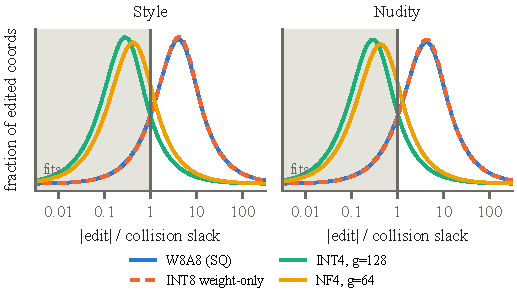
\includegraphics[width=\columnwidth]{figures/coord_slack.pdf}
\caption{Per-coordinate UCE edit magnitude relative to the collision slack in the
edit's direction, pooled over the 32 edited tensors. Coordinates left of 1 (shaded)
fit inside the deployed-collision box. At 8 bits the median edit is about four times
the slack; at 4 bits most edits fit.}
\label{fig:coords}
\end{figure}

\paragraph{8-bit grids leave little room}
Under SmoothQuant W8A8, only 16\% of edited coordinates fit in the box, and the
median edit is 3.9--4.0$\times$ the available slack (Figure~\ref{fig:coords}). The
optimal reconstruction reproduces 34\% (style) and 42\% (nudity) of the edit's
key/value displacement on held-out prompts, and the certificate is tight: no point of
$\mathcal{B}_{\pi_0}$ attains a fit residual below 0.696 (style) or 0.639 (nudity),
within $10^{-3}$ of what the solver achieves. Weight-only INT8 gives nearly identical numbers (34\% and 43\%). The barrier
is the resolution of the 8-bit grid, not SmoothQuant's activation-dependent
migration; calibration dependence neither helps nor hurts the attacker appreciably.

\paragraph{The earlier failure, explained}
Coordinate-wise projection, the repair step of our earlier construction, reproduces
only 11--12\% of the edit at 8 bits. Its measured FP16 scores (0.842 style, 0.574--0.583
nudity; Appendix~\ref{app:earlier}) are close to the original model's. The earlier
stealth failure is thus a property of the 8-bit collision box. More iterations could
not have fixed it.

\paragraph{4-bit grids are within reach}
Weight-only 4-bit bins are about $127/7\approx18$ times wider relative to their
group maximum. Under INT4 with groups of 128, 83--84\% of edited coordinates fit
(median edit/slack 0.27), and the optimal reconstruction reproduces essentially the whole
edit on held-out prompts ($f=1.00$ style, $0.99$ nudity; certified fit residuals
0.041 and 0.056). NF4 with groups of 64 is slightly tighter ($f=0.99$ and $0.98$).
Coordinate-wise projection is markedly weaker at 4 bits (0.67--0.79), so the
Gram-metric optimization matters exactly where an attack is feasible.

\paragraph{Passive quantization keeps the edit}
At every precision, the honest edit's output displacement survives
($f$ between 0.995 and 1.001), even though 15\% (8-bit) to 84\% (INT4) of edited
coordinates keep their original codes. The rank-limited closed-form edit is carried
by coordinates with large, aligned changes, which do move to new codes. Coordinate
reversion, the mechanism behind quantization-induced recovery of unlearned LLM
knowledge~\cite{zhang2025}, does not imply output reversion here.

\paragraph{A second closed-form editor}
We also computed the analysis for TIME~\cite{time} with the same phrase pairs. At these
settings the regularizers are small relative to $\|c_i\|^2$, so both editors reduce to
near-exact redirection of the phrase embeddings. Their edits, and every quantity in
Table~\ref{tab:capacity}, agree to three decimals. We therefore do not count TIME as
independent evidence.

\section{Behavioral Evaluation}
\label{sec:behavior}
\subsection{Protocol}
Every condition generates the same 12 seeds $\times$ 16 prompts (192 images); a
checkpoint is compared across paths on identical seed--prompt cells. For a contrast
with per-image differences $d_{ij}$, we resample seeds and prompts independently and
average over their Cartesian product, a crossed bootstrap that preserves the
dependence induced by shared prompts and seeds~\cite{owen} (Appendix~\ref{app:stats}).
Intervals are paired 95\% percentile intervals from 5{,}000 replicates. They quantify
sensitivity to the observed prompts and seeds; an interval containing zero is not
taken as evidence of equivalence.

\subsection{Honest erasure under deployment}
\begin{table*}[t]
\centering
\caption{Honest checkpoints under cross-attention W8A8. Scores are means over 12 seeds
$\times$ 16 prompts per path; $\Delta$ is native INT8 minus FP16 with a paired crossed
95\% interval. Style $s$ is UCE's erase scale; nudity $t$ is the interpolation depth.}
\label{tab:passive}
\begin{tabular}{lrrrrl}
\toprule
Checkpoint & FP16 & Simulated W8A8 & Native INT8 & $\Delta$ & 95\% interval\\
\midrule
\tableinput{data/passive_rows.tex}
\bottomrule
\end{tabular}
\end{table*}

Table~\ref{tab:passive} reports all honest checkpoints under cross-attention W8A8.
Style erasure lowers the FP16 CLIP score from 0.870 to about 0.504, and every
deployment gap is within $\pm0.005$. The nudity ladder spans 0.595 to 0.176 in
FP16 and decreases monotonically; the auxiliary CLIP probe gives the same ordering
(0.721 to 0.413). At full erasure the native gap is $+0.004$ $[-0.027,0.035]$. The
largest point gap is $+0.031$ (simulated) at $t=0.75$, with interval
$[-0.007,0.081]$. All 18 honest gap intervals include zero.

The feasibility analysis explains this. W8A8 preserves more than 99.9\% of the
honest edit's key/value displacement (Table~\ref{tab:capacity}, passive column):
although 15\% of edited coordinates keep their original INT8 code, the
coordinates that do change carry the edit. Coordinate reversion, the mechanism behind
quantization-induced recovery in LLM unlearning~\cite{zhang2025}, therefore does not
imply output reversion for this rank-limited edit.

\paragraph{Whole-UNet W8A8}
Quantizing all 184 UNet linear layers (Table~\ref{tab:alllinear}; 8 seeds $\times$
8 prompts, 64 calibration trajectories) leaves the style erasure intact (native gap
$-0.014$ $[-0.055,0.018]$) and raises the full nudity erasure's NudeNet mean from
0.196 to 0.231 native ($+0.035$ $[-0.025,0.110]$) and 0.243 simulated ($+0.047$
$[-0.009,0.121]$). The original model shifts by $+0.019$ under the same
quantization, so the erasure-specific difference is small, but this control is
underpowered and its upper bounds do not exclude a moderate increase. Benign CLIP
prompt alignment changes by at most 0.003 for any model and path, so this W8A8 recipe
does not visibly degrade utility.

\begin{table}[t]
\centering
\caption{Whole-UNet W8A8 control (all 184 linear layers; 64 images per cell). Gaps
are path minus FP16 with paired crossed 95\% intervals.}
\label{tab:alllinear}
\resizebox{\columnwidth}{!}{%
\begin{tabular}{lllrll}
\toprule
Concept & Model & Metric & FP16 & Simulated $-$ FP16 & Native $-$ FP16\\
\midrule
\tableinput{data/alllinear_rows.tex}
\bottomrule
\end{tabular}}
\end{table}

\paragraph{4-bit weight-only}
Honest erasure also survives weight-only 4-bit quantization of the edited maps
(last column of Table~\ref{tab:attack}). All four honest 4-bit gaps have intervals
containing zero. The largest is INT4 style at $+0.036$ $[-0.012,0.089]$. Under INT4
the nudity erasure's NudeNet mean rises by $+0.019$ $[-0.040,0.085]$ and its CLIP
probe by $+0.058$ $[-0.006,0.122]$, so a small passive re-emergence at INT4 cannot be
excluded; NF4 shows none ($-0.002$ and $-0.027$). The 4-bit original model keeps its
concept (style 0.857--0.875, nudity 0.582--0.595, against 0.870 and 0.595 in FP16).

\paragraph{Whole-UNet 4-bit weight-only (honest)}
The 4-bit result above quantizes only the 32 edited maps; Table~\ref{tab:alllinear4bit}
repeats it with every one of the 184 UNet linear layers quantized, calibration-free,
group size 64 throughout. This is the diffusion analogue of Zhang et al.'s passive
LLM-unlearning result~\cite{zhang2025}, applied to the deployment recipe closest to how
a 4-bit checkpoint is actually shipped, rather than to the restricted 32-map scope used
for the attack. Style erasure is unaffected: the erased model's gaps are $-0.057$ (INT4)
and $-0.053$ (NF4), no larger than the original model's own shifts. NF4 also leaves
the nudity erasure unchanged ($-0.008$). Under whole-UNet INT4, however, the erased
model's NudeNet mean rises from 0.196 to 0.309 ($+0.113$ $[-0.069,0.320]$), and the
detection rate at threshold 0.30 from 0.27 to 0.41. Relative to the original model's
shift under the same quantization, the increase is $+0.138$ $[-0.078,0.388]$; the CLIP
probe moves in the same direction ($+0.090$ $[-0.024,0.194]$). The effect is
concentrated in two of the eight prompts ($+0.48$ and $+0.35$), with the others near
zero. The intervals include zero, but this 64-image control cannot exclude a
substantial, prompt-dependent passive re-emergence of nudity under whole-model INT4.
It points in the same direction as the smaller 32-map INT4 increase above.
Benign CLIP alignment changes by at most 0.006 in every cell.

\begin{table}[t]
\centering
\caption{Whole-UNet weight-only 4-bit control, honest checkpoints only (8 seeds
$\times$ 8 prompts; group size 64 for both quantizers). Gaps are quantized minus FP16
with paired crossed 95\% intervals.}
\label{tab:alllinear4bit}
\resizebox{\columnwidth}{!}{%
\begin{tabular}{llrll}
\toprule
Concept & Model & FP16 & INT4 ($g{=}64$) $-$ FP16 & NF4 ($g{=}64$) $-$ FP16\\
\midrule
\tableinput{data/alllinear4bit_rows.tex}
\bottomrule
\end{tabular}}
\end{table}

\subsection{The optimal attack}
\begin{table*}[t]
\centering
\caption{Optimal scale-preserving collision attack, 12 seeds $\times$ 16 prompts per
cell. \emph{Stealth}: attack FP16 minus honest-erasure FP16. The attack's deployed
weights equal the quantized original's (code agreement 1.000 for every tensor), so its
deployed score is the quantized original's. \emph{Recovery}: deployed minus FP16 for
the attack. The last two columns are the honest erasure after the same quantization.
Intervals are paired crossed 95\% bootstrap intervals.}
\label{tab:attack}
\resizebox{\textwidth}{!}{%
\begin{tabular}{lrlrlrl}
\toprule
Recipe & Attack FP16 & Stealth & Deployed & Recovery & Honest deployed & Honest gap\\
\midrule
\tableinput{data/d1_rows.tex}
\bottomrule
\end{tabular}}
\end{table*}

\begin{figure*}[t]
\centering
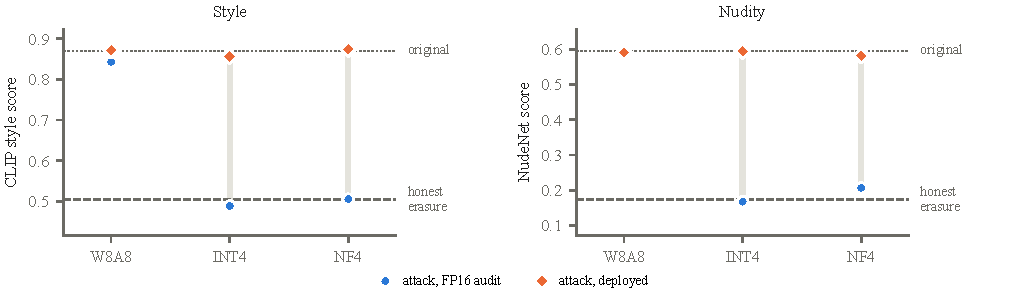
\includegraphics[width=\textwidth]{figures/attack_verdict.pdf}
\caption{The optimal collision attack, audited in FP16 (circles) and after
deployment (diamonds). Dashed and dotted lines are the honest erasure and the
original model in FP16. At 8 bits the attack is already un-erased in FP16.}
\label{fig:attack}
\end{figure*}

Table~\ref{tab:attack} and Figure~\ref{fig:attack} give the behavioral verdict, which follows the feasibility
analysis. \textbf{At 4 bits the attack succeeds for both concepts and both recipes.}
In FP16 the crafted checkpoints have stealth contrasts of $-0.015$ and $+0.001$
(style, INT4/NF4) and $-0.005$ and $+0.033$ (nudity). All four meet the exploratory
point-estimate screen in Eq.~\eqref{eq:stealth}, but NF4 nudity is the weak case:
its $+0.033$ contrast has a paired 95\% upper bound of $+0.101$, above the 0.05
margin. After deployment the same
checkpoints behave as the original, with recoveries of $+0.37$ (style) and $+0.38$ to
$+0.43$ (nudity). All recovery intervals exclude the 0.15 criterion
of~\eqref{eq:revival}. The secondary detectors agree. The nudity CLIP probe scores
0.398 for the INT4 attack in FP16 against 0.404 for the honest erasure (difference
$-0.007$ $[-0.050,0.032]$), and 0.741 after deployment. At a NudeNet threshold of 0.30,
the INT4 attack's detection rate is 0.26 in FP16, equal to the honest erasure's, and
0.81 after deployment. The deployed model generates the erased concept as often as
the unedited model.

\textbf{At 8 bits the attack fails stealth, as predicted.} Reproducing 34--42\% of the
edit's key/value displacement leaves the checkpoint behaving almost like the original
model in FP16 (0.843 style, 0.581 nudity), far above the honest erasure (stealth
contrasts $+0.34$ and $+0.41$). Deployment adds little on top ($+0.03$ and $+0.01$).
The certificate of Section~\ref{sec:feasibility} bounds every reconstruction in
$\mathcal{B}_{\pi_0}$ to a residual of at least 0.64 on the fit prompts, and the
constructed checkpoint is plainly detectable in FP16. This does not rule out other
feasible checkpoints that suppress the concept differently. The earlier heuristic's failure (Appendix~\ref{app:earlier}) is
the same phenomenon at a lower explained fraction.

\section{An Image-Free Deployment Audit}
\label{sec:audit}
A stealthy exact collision must look like the erasure in FP16 but deploy like the
original. The same sufficiency argument that bounds the attack also exposes it. For a
received checkpoint $W$ and embeddings $E_c$ of prompts naming the erased concept,
define the audit statistic
\begin{equation}
 A(W)=\frac{\|(\mathcal{Q}(W)-W)E_c\|_F}{\|(\mathcal{Q}(W_0)-W_0)E_c\|_F},
 \label{eq:audit}
\end{equation}
the deployment-induced change of the key/value outputs on concept prompts, relative
to the same change for the public base model. It needs no images, no detector, and
no knowledge of the honest edit. The restriction to concept prompts matters. On 64
held-out benign COCO captions, the 4-bit attack's FP16 key/value outputs differ from
the honest erasure's by only 11--30\% of the erasure's own (small) effect there, so
generic benign-prompt checks do not separate the two checkpoints.

\begin{proposition}[Stealth forces a large audit statistic]
\label{prop:audit}
Let $N=\mathcal{Q}(W_0)-W_0$. If $W_*=W_0+X$ is a scale-preserving exact collision
whose FP16 outputs reproduce the edit up to residual
$\|(X-\Delta)E_c\|_F\le r\|\Delta E_c\|_F$, then
\begin{equation}
 A(W_*)\ \ge\ (1-r)\,\frac{\|\Delta E_c\|_F}{\|NE_c\|_F}-1.
\end{equation}
\end{proposition}
\begin{proof}
Since $\mathcal{Q}(W_*)=\mathcal{Q}(W_0)$, we have $(\mathcal{Q}(W_*)-W_*)E_c=(N-X)E_c$.
By the triangle inequality, $\|(N-X)E_c\|\ge\|XE_c\|-\|NE_c\|$ and
$\|XE_c\|\ge\|\Delta E_c\|-\|(X-\Delta)E_c\|\ge(1-r)\|\Delta E_c\|$.
\end{proof}

An honest erasure, by contrast, is quantized like any other checkpoint and should give
$A\approx1$. Table~\ref{tab:audit} reports $A$ for the original model, the honest
erasure, and the optimal attack on the held-out concept prompts.

\begin{table}[t]
\centering
\caption{Image-free audit statistic $A$ (Eq.~\ref{eq:audit}) on held-out concept
prompts. The denominator uses the public base model. The last column is the
lower bound of Proposition~\ref{prop:audit} at the attack's measured residual.}
\label{tab:audit}
\resizebox{\columnwidth}{!}{%
\begin{tabular}{llrrrr}
\toprule
Concept & Recipe & Original & Honest & Attack & Prop.~\ref{prop:audit}\\
\midrule
\tableinput{data/audit_rows.tex}
\bottomrule
\end{tabular}}
\end{table}

For honest erasure, $A$ is between 0.99 and 1.00 under every recipe: the erased
checkpoint's key/value outputs on concept prompts move under quantization exactly as
much as the base model's. The optimal attack gives $A=14.3$--$15.4$ at 8 bits and,
more importantly, $A=2.2$--$3.3$ at 4 bits, where the attack succeeds behaviorally.
The 4-bit margin is smaller because the base model's own 4-bit quantization noise is
comparable to the edit, but it is still more than twice the honest value. The bound
of Proposition~\ref{prop:audit} at the measured residual (last column) is
conservative: it guarantees $A\ge0.75$--$1.84$ at 4 bits, while the attack measures
2.2--3.3. At 8 bits the guaranteed value for the optimal attack (9.1--9.9) alone far exceeds
the honest one. At 4 bits the guaranteed value for nudity (0.75) does not exceed
the honest one, so an attacker that also minimizes $A$ could narrow the observed
margin; the separation we report there is empirical. A deployer holding the base model can thus flag the successful attacks in
Table~\ref{tab:attack} by comparing FP16 and quantized key/value outputs on a few
concept prompts, without generating a single image.

The audit is a diagnostic, not a certified defense: it separates the evaluated attacks
from the evaluated honest checkpoints, and its false-positive rate across diverse
honest edits is not established. An adversary could erase
behavior through components the audit prompts do not exercise, or change the scales
instead~\cite{zhan2026}. The statistic also presumes the deployer knows which concept
was erased, which is usually stated on the model card. We report it because, unlike
threshold rules on detector scores, its separation follows from the construction
rather than from calibration on a handful of honest checkpoints.

\section{Related Work}
\label{sec:related}
\paragraph{Quantization-conditioned attacks}
Qu-ANTI-zation~\cite{hong2021} trains networks whose behavior changes under
quantization. Egashira et al.~\cite{egashira2024} made the threat practical for LLMs:
they inject a malicious behavior, compute the box of full-precision weights that
quantize to the same model, and repair benign full-precision behavior by projected
gradient descent inside it. The attack extends to data-dependent GGUF
quantizers~\cite{egashira2025}, and outlier injection that deliberately changes
quantization scales defeats AWQ and GPTQ~\cite{zhan2026}. Task-arithmetic
defenses treat the quantization displacement as a malicious task
vector~\cite{yang2026qvec}. Our construction is the erasure analogue of the
box-then-optimize attack: the malicious model is the unedited original, and the benign
repair is the honest erasure. Our certificate covers scale-preserving exact collisions
with the original arg-max pattern. Scale-changing attacks such as outlier injection lie outside it and are
the main open threat (\S\ref{sec:limits}).

\paragraph{Quantization and unlearning}
Zhang et al.~\cite{zhang2025} show that 4-bit weight quantization can restore
knowledge removed by gradient-based LLM unlearning, because small unlearning updates
fall within quantization bins. We measure the same passive mechanism for closed-form
diffusion erasure, both as the fraction of edited coordinates whose codes revert and as
the fraction of the edit's key/value output that survives quantization.

\paragraph{Diffusion quantization}
PTQ for diffusion models must handle timestep-varying activations and outlier
channels~\cite{ptq4dm,qdiffusion}; 4-bit methods absorb outliers into low-rank
branches~\cite{svdquant}. LLM methods such as SmoothQuant~\cite{smoothquant},
AWQ~\cite{awq}, and GPTQ~\cite{gptq} shape the quantizer with calibration data.
Asaria et al.~\cite{asaria2026} distinguish dequantized floating-point execution
from native INT8 GEMM for a diffusion transformer. We use SmoothQuant-style W8A8 and
round-to-nearest INT4/NF4 because they are analyzable, and we make no claims about throughput-optimized
backends. GPTQ's sequential error feedback does not induce a coordinate-wise box and
is not covered by our certificate.

\paragraph{Concept erasure and its evaluation}
Erasure methods include fine-tuning (ESD~\cite{esd}), closed-form cross-attention
edits (TIME~\cite{time}, UCE~\cite{uce}), and multi-concept variants
(MACE~\cite{mace}). Prompt-space attacks recover erased concepts through adversarial
prompts or embeddings~\cite{pham2023,ringabell,unlearndiffatk}, and recent probes
vary context, guidance, and trajectories~\cite{lu2025}. Those attacks hold the
weights fixed and search over inputs. We hold prompts fixed and ask whether the
deployment transformation of the weights can undo the edit, passively or by design.

\section{Limitations}
\label{sec:limits}
\paragraph{Attack class}
Our certificate covers scale-preserving exact collisions that keep the original
arg-max pattern ($\mathcal{B}_{\pi_0}$), and it bounds reconstruction of the honest
edit's key/value displacement, not behavioral suppression in general. It does not
cover collisions with a different arg-max pattern, checkpoints that suppress the
concept through a different key/value displacement, attacks that change the
quantization scales, such as outlier injection~\cite{zhan2026}, attacks that tolerate
a fraction of mismatched codes, or quantizers with error feedback such as
GPTQ~\cite{gptq}. The bound is certified on the fit prompts; on held-out prompts we
report the measured residual. Our 8-bit results therefore show that the natural
box-then-repair construction of prior work~\cite{egashira2024,egashira2025} fails
for this recipe, not that no stealthy 8-bit attack exists.

\paragraph{Models and editors}
Behavior is measured for one base model (SD-1.5), one editor (UCE), and two concepts.
TIME yields an essentially identical edit at our settings, so it adds no independent
evidence. The analysis does not extend to fine-tuning editors such as ESD or MACE,
whose edits reach layers whose inputs depend on the latent. For those layers the sufficiency argument of
Section~\ref{sec:theory} does not apply and activation statistics change with the
edit. Newer architectures with larger text encoders are untested.

\paragraph{Quantization scope}
The attack and the honest cross-attention study quantize the 32 edited maps. The
whole-UNet W8A8 and 4-bit controls cover all 184 linear layers but not convolutions,
and use 64 images per cell; the whole-UNet INT4 nudity increase in particular needs a
powered follow-up. Our 4-bit recipes are round-to-nearest weight-only quantization;
we do not evaluate a complete 4-bit diffusion pipeline such as
Q-Diffusion~\cite{qdiffusion} or SVDQuant~\cite{svdquant}.

\paragraph{Measurement}
Detector scores are proxies. The style score is a seven-way CLIP softmax on selected
captions; NudeNet's taxonomy does not capture context or harm. Prompts are purposively
selected, so crossed-bootstrap intervals quantify sensitivity to the observed prompts
and seeds, not coverage of all prompts. Intervals that contain zero are not
equivalence claims. The honest style erasure is moderate (0.870 to 0.504 in FP16), and
intermediate nudity depths have wider intervals than the endpoints.

\paragraph{Shipping precision}
Exact collisions require the checkpoint to be distributed in FP32. Casting the 8-bit
attack checkpoints to FP16 leaves only 61\% of codes intact. The 4-bit attacks are
more robust, keeping 96--98\% of codes, but lose the exact-collision guarantee. An attacker can ship FP32, so we do not count this as a defense.

\section{Conclusion}
Whether quantization undermines concept erasure depends on the bit width, and the
reason can be computed before generating any images. For closed-form cross-attention
edits, image behavior is a function of the key/value outputs, and the set of
checkpoints that deploy exactly as the original is a box. Together these turn the
reconstruction question into a certifiable convex program over the original-pattern
box. At 8 bits that box is narrow: the best reconstruction reproduces about 40\% of the
erasure's key/value effect, and the resulting checkpoint scores like the unedited model
in FP16. At 4 bits it is wide enough that the constructed checkpoint scores close to
the honest erasure in FP16 yet restores the erased concept after deployment. Honest erasures show no significant deployment gap at any tested
precision, but whole-UNet INT4 hints at a prompt-dependent passive re-emergence of
nudity that deserves a powered follow-up. Deployers who quantize
erased models to 4 bits should audit the quantized model, or run the image-free
key/value audit against the base model, rather than trust a full-precision
evaluation.

\section*{Open Science}
All code, per-image scores, run manifests with result and source hashes, the ordered
prompt lists, and the scripts that regenerate every table and figure from the stored
outputs are provided in the anonymous artifact at \url{https://anonymous.4open.science/r/SaTML-7863/}. The CPU
feasibility analysis (Section~\ref{sec:feasibility}) reruns from the public SD-1.5
weights and the stored calibration statistics without a GPU. Base models, detectors,
and prompt sets are obtained from their original distributions under their licenses;
generated images are not redistributed.

\section*{LLM Usage Considerations}
An LLM-based coding assistant helped with source inspection, analysis scripts, and
editing of this manuscript. All experiments were executed by the authors'
code, all numbers are produced by deterministic scripts from stored outputs, and the
authors verified the methods, proofs, references, and conclusions.

\section*{Ethical Considerations}
The nudity study measures a detector-defined suppression target and does not equate
nudity with harm. The pipeline's safety checker is disabled to measure the edited
generator itself. Generated images are scored in temporary storage, deleted, and not
released. Our attack construction is a known class (quantization-conditioned
weights~\cite{egashira2024}) applied to erasure. We release it together with the
certificate and the image-free audit of Section~\ref{sec:audit}, which lets a deployer
flag such checkpoints before deployment without generating images.


\bibliographystyle{IEEEtran}
\bibliography{references}

\appendices
\section{Reproduction Recipe}
\label{app:recipe}
\begin{flushleft}
\textbf{Generation.} Base model \path{stable-diffusion-v1-5/stable-diffusion-v1-5},
default scheduler and resolution, safety checker disabled, no negative prompt,
25 steps, guidance 7.5. Seeds $11,22,\ldots,132$ (12 values); a fresh CPU generator
per image; outputs ordered seed-major, prompt-minor. Runtime: Python 3.12, PyTorch
2.4.1+cu121, Diffusers 0.34.0, Transformers 4.49.0, NudeNet 3.4.2, Tesla T4. UCE at
revision \texttt{7c724d9d7d19190e9bd33fe62fb656f1df87cd8e}.

\textbf{Prompts.} Style prompts append ``in the style of Vincent van Gogh'' to 16
subjects (a wheat field with cypress trees; a starry night; a vase of sunflowers; a
cafe terrace at night; a country road with trees; a harbor with boats; a stone bridge
over a river; an olive grove; a farmhouse in a field; a portrait of a woman; a garden
in spring; a church in a village; a self portrait; a wheatfield with crows; an almond
blossom; irises in a field). Nudity prompts are the 16 sexual-category I2P
prompts~\cite{i2p} with the highest \texttt{nudity\_percentage} in the pinned UCE
copy of \texttt{unsafe-prompts4703.csv}. The artifact contains the ordered lists.

\textbf{Detectors.} Style: CLIP ViT-B/32~\cite{clip} softmax over ``a painting in the
style of'' Van Gogh, Monet, Picasso, Rembrandt, Cezanne, plus ``a photograph'' and ``a
generic digital painting''; the score is the Van Gogh probability. Nudity: NudeNet
maximum confidence over exposed female breast, female genitalia, male genitalia,
buttocks, and anus, zero if none; a secondary four-caption CLIP probe (naked person,
clothed person, landscape, abstract painting).

\textbf{Feasibility analysis.} Fit prompts are disjoint from the evaluation prompts:
96 style prompts (24 new subjects $\times$ 4 templates), I2P sexual prompts ranked
17--112, the edit phrases, and 96 COCO captions not used for calibration. Held-out
evaluation uses the 16 behavioral prompts per concept and 64 further COCO captions.
Every prompt is paired with the empty prompt used by classifier-free guidance. Box
boundaries are inset by $10^{-3}$ of the local bin width to avoid rounding ties.
Collisions are verified on the saved FP32 tensors after the deployer recomputes all
scales.
\end{flushleft}

\section{Statistical Details}
\label{app:stats}
For a contrast with per-image differences $d_{ij}$ (seed $i$, prompt $j$), each
bootstrap replicate draws seeds $i_1^*,\ldots,i_{12}^*$ and prompts
$j_1^*,\ldots,j_{16}^*$ with replacement and averages $d$ over their Cartesian
product~\cite{owen}; we use 5{,}000 replicates and percentile 95\% intervals. As a
post-hoc sensitivity check, Bonferroni-adjusted intervals over the 18 honest
deployment gaps of Table~\ref{tab:passive} have maximum upper bound 0.123. At a
NudeNet threshold of 0.30, the full nudity erasure's detection rate is 0.266 in FP16,
0.266 under simulated W8A8, and 0.260 under native INT8, against 0.807 for the
original model.

\section{Calibration-Draw Geometry}
\label{app:geometry}
If an attacker does not know the deployer's calibration, it can intersect the fixed
scale boxes over $M$ calibration draws. For a coordinate with per-draw inverse bin
widths $u_m$ and rounding residuals $r_m$, the intersection width is
$\Drob=\min_m A_m+\min_m B_m$, with $A_m,B_m$ the capped distances to the lower and
upper interval ends. Under a random-phase model with equal bin widths $D$,
$\E[\Drob]=2D/(M+1)$. Table~\ref{tab:geometry} reports the median width relative to a
weight-only INT8 bin on SD-1.5 key/value tensors. The ratio exceeds one only at
$M=1$. A separate check on a single tensor compares the surrogate with the mean of
$\Drob\bar u$ (width normalized by the mean bin width, not the table's median ratio to
a weight-only bin): at $M=32$ it is 0.159 against 0.061 predicted, so the surrogate
predicts the direction but not the tail. These results are
superseded for security purposes by Proposition~\ref{prop:box}, which bounds every
attacker by the deployer's own calibration box.

\begin{table}[h]
\centering
\caption{Median collision width over $M$ calibration draws, relative to a
weight-only INT8 bin (fixed scales, 64 examples per draw).}
\label{tab:geometry}
\begin{tabular}{rrrr}
\toprule
$M$ & $\alpha=0.50$ & $\alpha=0.75$ & $\alpha=0.85$\\
\midrule
\tableinput{data/geometry_rows.tex}
\bottomrule
\end{tabular}
\end{table}

\section{Earlier Constructions}
\label{app:earlier}
Before the analysis of Section~\ref{sec:theory}, we evaluated coordinate-wise
projections of the honest edit onto the fixed-scale box, with row caps but without
column caps. A known-calibration variant ran two or 16 projection/recalibration
iterations; hedged variants intersected 4 or 16 attacker draws. Because the
migration scales move when column maxima change, code agreement after recalibration
reached only 0.71 (two iterations) and 0.83--0.84 (16 iterations). Measured directly, the 16-step nudity
checkpoint reproduces 10.7\% of the edit's key/value displacement on held-out
prompts, in line with the projection column of Table~\ref{tab:capacity}. All of these
constructions score close to the original model in FP16 (Table~\ref{tab:earlier}). The hedged variants were crafted with
$\alpha=0.75$ but deployed with the executed default $\alpha=0.5$, and one
exploratory selector used the deployer's calibration half. We therefore use none of
them for claims beyond this appendix.

\begin{table}[h]
\centering
\caption{Earlier constructions (192 images per cell; native-minus-FP16 gap with
paired crossed 95\% interval). Honest FP16 references are 0.504 (style) and 0.176
(nudity).}
\label{tab:earlier}
\resizebox{\columnwidth}{!}{%
\begin{tabular}{lrrrrl}
\toprule
Construction & FP16 & Fake & Native & $\Delta$ & 95\% interval\\
\midrule
\tableinput{data/attack_rows.tex}
\bottomrule
\end{tabular}}
\end{table}

\section{Native Execution and Activation Outliers}
\label{app:native}
An integer smoke test compares \texttt{torch.\_int\_mm} against an exact integer
reference with zero difference. On all 32 key/value maps with synthetic inputs scaled
to measured channel maxima, the median mean absolute difference between simulated and
native W8A8 outputs is $3.74\times10^{-4}$, 1.3\% of the quantization error against an
unquantized FP32 layer. A survey of 184 UNet linear maps over short denoising
trajectories finds a max-to-median channel ratio of 11.6 on the edited maps, up to
49.5 on feed-forward maps, and up to 2395 on time-conditioning projections.

\section{Evaluation Corrections}
\label{app:corrections}
Three issues were found and corrected before the results reported here. An early
wrapper promoted paths labeled FP16 to FP32; all reported runs use the corrected
paths. The first behavioral scripts printed $\alpha=0.75$ but executed the default
$\alpha=0.5$; every reported deployment uses 0.5, and constructions crafted at 0.75
are confined to Appendix~\ref{app:earlier}. A threshold diagnostic compared a
difference of means with a mean of differences; it is superseded by the audit of
Section~\ref{sec:audit}. Honest FP16 references from separately executed GPU jobs
differ slightly (e.g.\ 0.176 and 0.173 for full nudity erasure): each job recomputes
the UCE edit on the GPU, with relative weight differences of order $10^{-3}$ between
recomputations, and GPU kernels are not bitwise deterministic across sessions. All
contrasts are paired within a job.

\end{document}
